\section{Use Cases} \label{sec:UseCases}

Various methods of XAI have been layed out in the previous section, but the question still remains of how do these methods provide value to scientists, consumers, or society at large.  Here, we explore the various users who interface with XAI and what value is provided.

\subsection{As a data scientist, I can use the explanation of a model's decisions to identify opportunities to improve the training data set and make the model more robust}\label{subsec:UseCase1}

This use case takes an \textit{a posteriori} approach to identifying opportunities to improve a model's performance.  In current literature, the XAI methods involved are commonly visualization techniques, but other methods are still applicable.  Due to the subjective nature of interpretation methods like visualization of relevant features, any action in improving the training of a model requires a human expert to analyze the explanation for potential weaknesses in the model's decision process.

In one example of improving a model through the identification of relevant features, a group of researchers used a Fisher Vector classifier on the PASCAL VOC 2007 data set \cite{Bach2016AnalyzingCF}.  After applying LRP to as a tool in explaining the classifier's decisions, it was apparent that the copyright watermark on images of horses was highly relevant in the Fisher Vector model.  The researchers then removed the copyright watermark before retraining the model, and future decisions considered the horse and its surroundings as more relevant features (see figure \ref{fig:bach2016}).

\begin{figure}
    \centering
    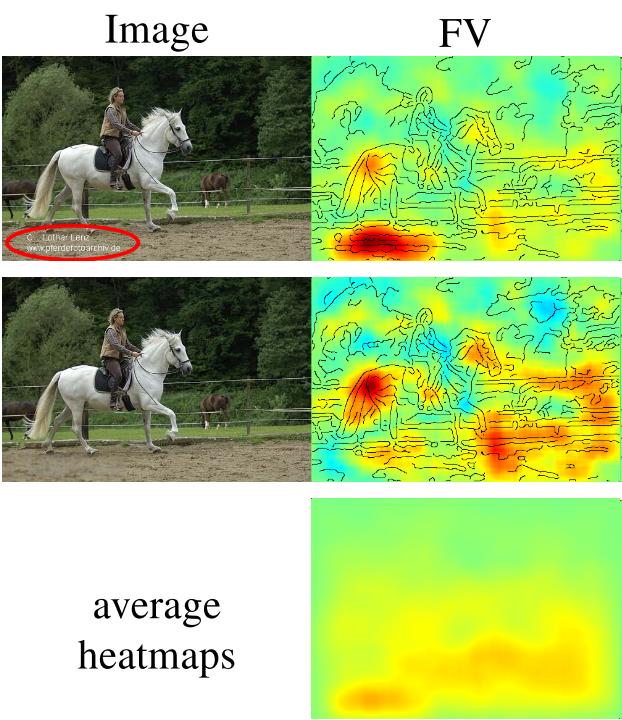
\includegraphics[width=3.4in]{media/bach2016.png}
    \caption{Heatmaps generated via LRP for a Fisher Vector classifier, before and after the removal of a watermark from the training data. \cite{Bach2016AnalyzingCF}.}
    \label{fig:bach2016}
\end{figure}

\subsection{As a potential consumer of an AI/ML product, such as an autonomous vehicle or virtual assistant, an explanation of how the product is making its decisions will improve my trust in the product}\label{subsec:UseCase2}

The psychological study of the trustworthiness of AI systems is as old as AI itself, but there are recent contributions to how XAI contributes to people's perceptions of ML models and decision systems.  Ribeiro et al. trained a classifier of images of wolves and huskies with intentionally biased training data and measured human subjects' trust in the model before and after receiving an explanation of a misclassified input \cite{Ribeiro:2016:WIT:2939672.2939778}.  The classifier was trained with images that were hand selected such that images of wolves had snow in the background and images of huskies did not.  Human subjects observing the classifications and receiving the explanation were all students in an ML course, so each participant had a background in black-box models.  Before receiving an explanation of a misclassification from the model as seen in figure \ref{fig:ribeiro2016}, 10 out of 27 students trusted the model, but after the students received an explanation of the model's decision, only 3 of the students reported trusting the model.  While the sample size of human subjects is small and limited to a very specific demographic, the result is intuitive that an explanation of a misclassification from a biased model directly impacts the trust in that model.  In a similarly small experiment, Koo et al. establish that users of a vehicle simulator had more positive emotional responses when a driving-assistance system provided explanations for when it applied hard break events in emergency scenarios \cite{Koo2015}.

\begin{figure}
    \centering
    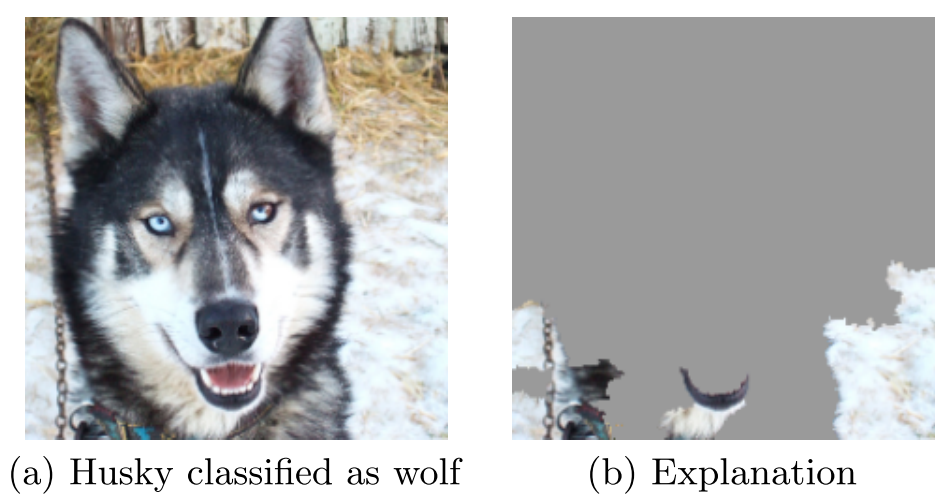
\includegraphics[width=3.4in]{media/ribeiro2016.png}
    \caption{Heatmaps generated via LRP for a Fisher Vector classifier, before and after the removal of a watermark from the training data. \cite{Ribeiro:2016:WIT:2939672.2939778}.}
    \label{fig:ribeiro2016}
\end{figure}

\subsection{As a provider of an AI/ML product, I am responsible for providing an explanation for how my product makes its decisions in the case of being the subject of scrutiny, legal or otherwise}\label{subsec:UseCase3}

While legislation such as the EU's General Data Protection Regulation's "right to explanation" faces legitimate criticism about its scope and ability to be enforced \cite{Mittelstadt2017}, there also exists an ethical imperative for providers of AI/ML products to provide explanations for their systems' decisions.  For example, in the criminal justice system, judges and parole boards may apply predictive models as tools in making their decisions, but racial discrimination has been uncovered in such tools \cite{Wexler.2017} \cite{Angwin2016}.  While there is a lack of enforceable legislation around regulating the accountability of automated decision systems, autonomous vehicles and vehicles with ADAS from Tesla, Google, and GM Cruise have been involved with numerous traffic incidents, ranging from trivial to fatal \cite{Read2016} \cite{Tesla2018} \cite{Ackerman2016} \cite{Bhavsar2017}.  It may be commercially advantageous for automakers to continue to push the capabilities of technology by designing autonomous systems that can provide effective explanations to various stakeholders before legislation and regulations require it of autonomous vehicles.
